\documentclass[]{article}

\RequirePackage[utf8]{inputenc}
\RequirePackage[french,english]{babel}

\newif\ifthesis
\thesisfalse

\usepackage{amsmath}
\usepackage{amsfonts}
\DeclareMathOperator{\Lapl}{\mathcal{L}}
\DeclareMathOperator{\bigO}{\mathcal{O}}
\DeclareMathOperator{\Real}{\mathbb{R}}

\usepackage[bottom]{footmisc}

\usepackage[backend=bibtex, style=numeric, sorting=none]{biblatex}
\addbibresource{references.bib}

\usepackage{graphicx}
\usepackage{subcaption}
\usepackage{float}
\usepackage{pgfplots}
\usepgfplotslibrary{groupplots}

\usepackage{algorithm}
\usepackage{algorithmic}
\renewcommand{\algorithmicrequire}{\bf{Input:}}
\renewcommand{\algorithmicensure}{\bf{Output:}}

\usepackage{enumitem}
\usepackage{hyperref}

\title{Image Processing using Graph Laplacian Operator}

\author{David Wobrock \\ \texttt{david.wobrock@gmail.com}}
\date{\today}

\begin{document}

\maketitle

Under the responsability of:\\ \\
Supervisor: Frédéric Nataf\\
ALPINES Team - INRIA Paris\\
Laboratoire Jacques-Louis Lions - Sorbonne Université \\ \\
INSA Supervisor: Christine Solnon\\
Département Informatique\\
INSA de Lyon

\begin{abstract}
 The latest image processing methods are based on global data-dependent filters.
These methods involve huge affinity matrices which cannot fit in memory and need to be approximated using spectral decomposition.
The inferred eigenvalue problem concerns the smallest eigenvalues of the Laplacian operator which can be solved using the inverse iteration method which, in turn, involves solving linear systems.
In this master thesis, we detail the functioning of the spectral algorithm for image editing and explore the behaviour of solving large and dense systems of linear equations in parallel, in the context of image processing.
We use Krylov type solvers, such as GMRES, and precondition them using domain decomposition methods to solve the systems on high-performance clusters.
The experiments show that Schwarz methods as preconditioner scale well as we increase the number of processors.
However, we observe that the limiting factor is the Gram-Schmidt orthogonalisation procedure.
We also compare the performances to the state-of-the-art Krylov-Schur algorithm provided by the SLEPc library.

\end{abstract}

\paragraph{Keywords}
image processing, graph Laplacian operator, eigenvalue problem, high performance computing

\begin{otherlanguage}{french}
  \begin{abstract}
   Les plus récentes méthodes de traitement d'images sont basées sur des filtres globaux dépendant des données.
Ces méthodes impliquent d'immenses matrices de similarités et de Laplacien de graphe de l'image en entrée.
Puisque ces matrices ne tiennent pas en mémoire, il est nécessaire de les approcher par l'échantillonnage et l'extension de Nystr\"om basée sur la décomposition spectral des matrices.
Le problème aux valeurs propres qui en découle concerne les plus grandes valeurs propres du filtre.
Néanmoins, celle-ci corresponde aux plus petites valeurs propres du Laplacien.
Pour résoudre ce problème, nous utilisons la méthode la puissance inverse, qui converge mieux dans ce cas, mais qui implique la résolution de systèmes linéaires.
Dans cette thèse de master, nous étudions le comportement de la résolution de systèmes d'équations linéaires sur de grandes matrices pleines, dans le cadre du traitement d'images, en utilisant des méthodes de décomposition de domaines comme préconditionneur.
Les expériences montrent que les méthodes de type Krylov combinées avec les méthodes de Schwarz comme préconditionneur passe bien à l'échelle pour de grandes systèmes linéaires avec des matrices pleines.

  \end{abstract}
\end{otherlanguage}

\paragraph{Mots-clés}
traitement d'images, Laplacien graphe, problème aux valeurs propres, calcul haute performance

\section{Introduction}

\subsection{Background}
\paragraph{}
The talk \cite{siam_slides_2016} and articles \cite{glide_2014} \cite{talebi_nonlocal_2014} by Milanfar, working at Google Research, about using the graph Laplacian operator for nonconformist image processing purposes awakes curiosity.

Indeed, Milanfar reports that these techniques to build image filters are used on smartphones, which implies a reasonable execution time with limited computational resources.
Over 2 billion photos are shared daily on social media \cite{siam_slides_2016}, with very high resolutions and most of the time some processing or filter is applied to them.
The algorithm must be efficient to be deployed at such scale.


\subsection{Objective}
\paragraph{}
The aim of this degree project is not to explore and improve the state of image processing.
Instead, the spectral methods used in the algorithm will be our focus point.
Those will inevitably expose eigenvalue problems, which may involve solving systems of linear equations.

Concerning the challenges about solving linear systems, on the one hand, the size of the systems can be large when considering high-resolution images with millions of pixels, or even considering 3D images.
We process huge matrices of size \(N^2\), with \(N\) the number of pixels of the input image.
On the other hand, those huge affinity matrices are dense, thus the linear systems are dense.
Often, linear systems result from discretising partial differential equations (PDEs) yielding sparse matrices, and therefore most linear solvers are specialised in sparse systems.

The aim of this work is to explore the performance of linear solvers on dense problems, their stability and convergence.
This will include preconditioning the linear systems, especially using domain decomposition methods, and analyse their behaviour on dense systems.


\section{Image processing using graph Laplacian operator}
\paragraph{}
A global image filter consists of a function which outputs one pixel, taking all pixels as input and applying weights to them.
\ifthesis
 Let \(z_i\) be the output pixel, \(W_{ij}\) the weights, \(y_j\) all input pixels and \(N\) the number of pixels in the image.
 We compute one output pixel with:
 \[z_i = \sum^{N}_{j=1} W_{ij}y_j,\]
 This means that a vector of weights exists for each pixel.
\fi

As a practical notation, we say that, with \(W\) the matrix of weights and \(y\) and \(z\) respectively the input and output images as vectors,
\[z = Wy.\]
The filter matrix \(W\) considered here is data-dependent and built upon the input image \(y\).
A more mathematical notation would consider \(W\) as a nonlinear function of the input image such as \(z = W(y) \cdot y\).


\paragraph{Image as graph}
Let's think of an image as a graph.
Each pixel is a node and has edges to other nodes.
The simplest way to connect pixels to other pixels is their direct neighbours, in which case each node has four edges.
To avoid losing any information, we will instead consider the case of a complete graph; each node connects to all other nodes.

To preserve the image information in the graph, the graph edges will be assigned a weight, measuring the similarity\footnote{Also called affinity.} between two nodes, thus between two pixels.

There are multiple ways the similarity can be defined.
The most intuitive definition considers spatial proximity.
This means that similar pixels are spatially close, which, translated to a basic filter, is the same as a Gaussian filter which computes a weighted average of the pixel's neighbourhood and produces what is known as Gaussian blur.
Another similarity definition is to consider the pixel's colour.
A good compromise is to consider an average of both, spatial and colour closeness, with a certain weighting.
\ifthesis
A summary of some affinity functions can be found in section \ref{variations:affinity_functions}.
\fi

Once the similarity is defined, we can compute the adjacency matrix of the graph including the edge weights.
This matrix is called the affinity matrix\footnote{Or similarity matrix, or kernel matrix}\ \(K\) which represents the similarity of each pixel to every other pixel in the image.
Consequently, this matrix is symmetric and of size \(N \times N\) with \(N\) the number of pixels in the image.
Also, most similarity functions define bounds on the values of \(K\) such as \(0 \le K_{ij} \le 1\).

Using this affinity matrix, we obtain the graph Laplacian \(\Lapl\), used to build the filter matrix \(W\).


\paragraph{Building the filter}
Multiple graph Laplacian definitions, more or less equivalent, exist and can have slightly different properties.
The table \ref{table:laplacians} proposes a summary of most Laplacian matrix definitions.
In the case of image smoothing, the filter \(W\) is roughly defined such as \(\Lapl = I - W\) \cite{siam_slides_2016} and so \(W = I - \Lapl\).
To get various filters using one Laplacian, we can apply some function \(f\) to \(\Lapl\) and obtain \(W = I - f(\Lapl)\) which gives us more possibilities on the filter computation.
Below the global filter algorithm if we compute the entire matrices:

\begin{algorithm}[H]
 \caption{Image processing using entire graph Laplacian operator}
 \begin{algorithmic}
  \REQUIRE \(y\) an image of size \(N\), \(f\) the function applied to \(\Lapl\)
  \ENSURE \(z\) the output image
  \STATE Compute \(K\) (size \(N \times N\))
  \STATE Compute Laplacian matrix \(\Lapl\)
  \STATE \(z \leftarrow (I - f(\Lapl)) y\)
 \end{algorithmic}
\end{algorithm}

However, all these matrices \(K\), \(\Lapl\) and \(W\) represent huge computational costs.
Only storing one of these matrices is already a challenge since they have a size of \(N^2\).

For example, a tiny test image of size \(256 \times 256\) has 65 536 pixels, so one of these matrices has approximately \(4.29 \times 10^9\) elements.
Considering storing those with a 64 bits type, one matrix takes more than 34 GB of memory.
Scaling to an everyday-smartphone picture, taken with a 10 MPixel camera, a matrix contains \(10^{14}\) elements, meaning 800 TB of memory for each matrix.


\paragraph{Approximation by sampling and Nystr\"om extension}
To avoid storing any of those huge matrices, approximation will be necessary.
Following \cite{fowlkes_spectral_2004}, we define the Nystr\"om extension.
It starts by sampling the image and only select a subset of \(p\) pixels, with \(p \ll N\).
Numerically, \(p\) should represent around 1\% or less of the image pixels.
\ifthesis
 The rows and columns of a matrix \(K\) are reorganised such as \(K_A\) the upper left affinity matrix of \(K\) of size \(p \times p\), measuring the affinities between the sampled pixels.
 The submatrix \(K_B\) is holding the similarities between the sampled pixels and the remaining pixels and is of size \(p \times (N-p)\).
 And the lower right submatrix \(K_C\) contains the affinities between the remaining pixels.
 We have:
 \[K = \begin{bmatrix}K_A & K_B \\ K_B^T & K_C\end{bmatrix}.\]
 Knowing that \(K_C\) is of size \((N-p) \times (N-p)\) and that \(p \ll N\), this submatrix is still huge and must be avoided.
 
 To have a numerical approximation of a symmetric (semi) positive definite matrix \(K\), we use the eigendecomposition with \(\Phi\) the orthonormal eigenvectors of \(K\) stored as a matrix and \(\Pi\) the eigenvalues of \(K\):
 \[K = \Phi \Pi \Phi^T.\]
 The article \cite{fowlkes_spectral_2004} suggests the Nystr\"om extension to approximate \(K\) by \(\tilde{K} = \tilde{\Phi} \tilde{\Pi} \tilde{\Phi^T}\), using the eigendecomposition of the submatrix \(K_A = \Phi_A \Pi_A \Phi_A^T\), with \(\tilde{\Pi} = \Pi_A\) and the approximated leading eigenvectors \(\tilde{\Phi}\):
 \begin{equation}
  \begin{split}
   \tilde{\Phi} & = \begin{bmatrix}\Phi_A \\ K_B^T K_A^{-1} \Phi_A \end{bmatrix} \\
                & = \begin{bmatrix}\Phi_A \\ K_B^T \Phi_A \Pi_A^{-1} \end{bmatrix}
  \end{split}
 \end{equation}
 We can calculate
 \begin{equation}
  \begin{split}
      \tilde{K} & = \tilde{\Phi} \tilde{\Pi} \tilde{\Phi^T} \\
                & = \begin{bmatrix} \Phi_A \\ K_B^T \Phi_A \Pi_A^{-1} \end{bmatrix} \Pi_A \begin{bmatrix} \Phi_A^T & \Pi_A^{-1} \Phi_A^T K_B \end{bmatrix} \\
                & = \begin{bmatrix} \Phi_A \Pi_A \\ K_B^T \Phi_A \end{bmatrix} \begin{bmatrix} \Phi_A^T & \Pi_A^{-1} \Phi_A^T K_B \end{bmatrix} \\
                & = \begin{bmatrix} K_A & K_B \\ K_B^T & K_B^T K_A^{-1} K_B \end{bmatrix}
  \end{split}
 \end{equation}
 
 We can clearly see that the huge submatrix \(K_C\) is now approximated by \(K_B^T K_A^{-1} K_B\).
 The quality of the approximation is measurable by the norm of the difference of the two above terms.
 We recognise the norm of the Schur complement \(\| K_C - K_B^T K_A^{-1} K_B \| \).
\else
 We only need to compute of subset of the affinity matrix \(K\) and then compute the eigendecomposition of a submatrix.
 The eigenvectors of the submatrix are extended to the entire matrix and used to reconstruct it.
\fi

Therefore, we will only need to compute two submatrices.
\ifthesis
 For our previous examples, if we sample 1\% of the pixels, we need to store 0.34 GB of data for each matrix, instead of 34 GB for the \(256 \times 256\) image.
 For a 10 megapixel image, each matrix needs 8 TB of memory, which is still a lot of memory.
 However, as \cite{fowlkes_spectral_2004} and \cite{glide_2014} propose, the sampling rate can be lower than 1\% and still contain most of the relevant image information.
\else
 For our previous example, for the 10 megapixel image, each matrix needs 8 TB of memory, which is still a lot of memory, but the sampling rate can be lower than 1\% as suggested by \cite{fowlkes_spectral_2004} and \cite{glide_2014}.
\fi


\paragraph{Eigendecomposition}
We need to compute the largest eigenvalues of the filter \(W\).
The reason can be found by formulating the filter by its diagonalisation \(W = \sum_i^N \lambda_i \phi_i \phi_i^T\).
When the \(i\)th eigenvalue \(\lambda_i\) is small, the eigenvector product will be negligible, and therefore the largest eigenvalues of the filter \(W\) are the most relevant.

For the approximation, we will actually need to compute the largest eigenvalues of the sampled pixels submatrix \(W_A\) to use the Nystr\"om extension.
Using a sample to compute the largest eigenvalues works to approximate the complete filter because these eigenvalues are decaying rapidly as shows the figure below:
\begin{figure}[H]
  \centering
  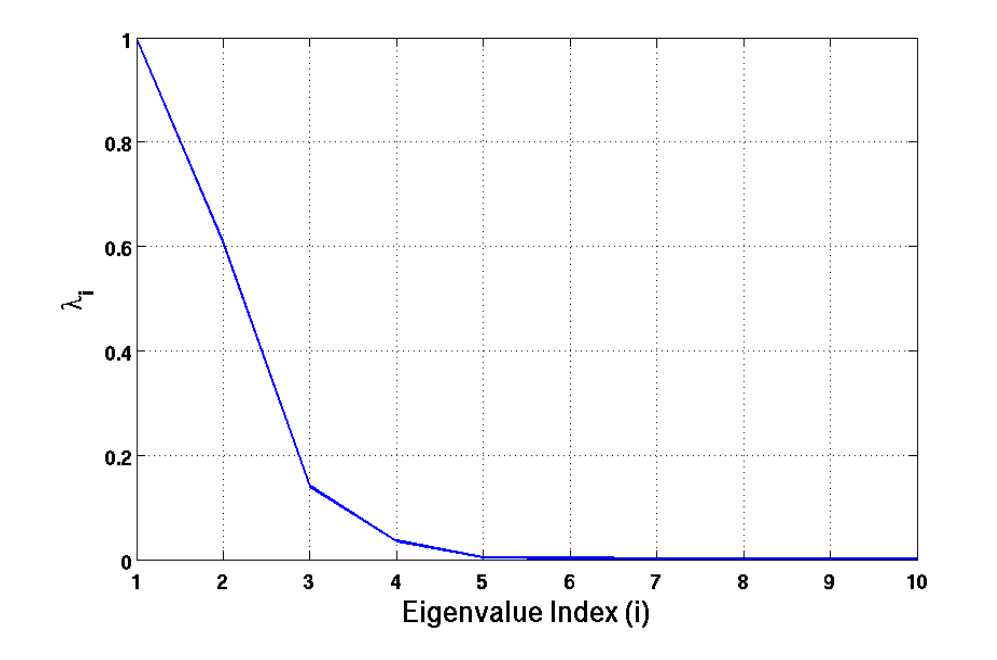
\includegraphics[width=0.9\textwidth]{img/decayingEigenvalues.png}
  \caption{Largest eigenvalues of an image filter, taken from \cite{siam_slides_2016}.}
\end{figure}
% TODO refaire soit meme

We know that the eigenvalues of submatrix\ \(W_A\) are between the extremum eigenvalues of the filter \(W\), which is known as the interlacing property of principal submatrices.
We also know that computing the largest eigenvalues of the submatrix filter is equivalent to computing the smallest eigenvalues of the corresponding Laplacian operator.
The proofs to these statements can be found in Appendix \ref{appendix:eigenvalue_proof}.

The goal of this observation is the way of computing the eigenvalues.
For the largest eigenvalues, the most famous algorithm is the power method.
For the smallest eigenvalues, the inverse power method is a usual choice.
Both methods converge faster when two successive eigenvalues are far from each other.
In our case, the largest eigenvalues are close to each other; hence the inverse of these eigenvalues will be far from each other.
We will therefore prefer the inverse power method.

The algorithm will, in an iterative manner, compute the associated eigenvector of an eigenvalue.
This requires either to invert a matrix such as \(x_{k+1} = A^{-1} x_k\), or to solve the linear system \(A x_{k+1} = x_k\).
We will solve systems of linear equations to compute the first eigenvalues of the Laplacian in order to observe the behaviour of solvers on these dense matrices.

The main drawback of the Nystr\"om method for us, is that it approximates the leading eigenvalues and we compute the trailing ones of the Laplacian \(\Lapl\) \cite{belongie_spectral_2002}.
It is possible to obtain the eigendecomposition of the filter \(W\), even when \(W\) is indefinite, through a method proposed by \cite{fowlkes_spectral_2004}.
It consists of computing the matrix \(W_A^{-1/2}\), which could be done either by the complete eigendecomposition or by using Cauchy's integral formula.
After this step, two more diagonalisation of matrices are required, demanding an important computation time.

Nevertheless, as stated in the objectives of the project, our main goal is not the image processing aspect, but the behaviour of linear solvers of these dense matrices using domain decomposition methods.
We will therefore stick to computing the smallest eigenvalues of the Laplacian operator \(\Lapl\) and avoid spending too much time on the end of the algorithm implementation.


\paragraph{}
\ifthesis
 Even if we cannot approximate the trailing eigenvectors of \(\Lapl\) through the eigenvectors of \(\Lapl_A\), we still define how the Laplacian is used to compute the output image.
 The summary \cite{modern_tour_2013} implicitly defines the filter as \(W = I - f(\Lapl)\) with the function \(f\) that helps achieving various filters.
 To apply the function efficiently to the Laplacian operator, we apply it to the diagonal eigenvalue matrix such as \(f(\Lapl) = \Phi f(\Pi) \Phi^T\).
 The output image using the filter approximation \(\tilde{W}\) can be expressed as:
 \begin{equation}
  \begin{split}
      \tilde{z} & = \tilde{W}y \\
                & = (I - f(\tilde{\Lapl})) y \\
                & = (I - \tilde{\Phi} f(\tilde{\Pi}) \tilde{\Phi^T}) y \\
                & = y - \tilde{\Phi} f(\tilde{\Pi}) \tilde{\Phi^T} y
  \end{split}
 \end{equation}
\fi

Below a summary of the complete algorithm using spectral decomposition of the matrix to approximate it:

\begin{algorithm}[H]
 \caption{Image processing using approximated graph Laplacian operator}
 \begin{algorithmic}
  \REQUIRE \(y\) an image of size \(N\), \(f\) the function applied to \(\Lapl\)
  \ENSURE \(\tilde{z}\) the output image by the approximated filter
  \STATE \COMMENT{Sampling}
  \STATE Sample \(p\) pixels, \(p \ll N\)
  \STATE \COMMENT{Kernel matrix approximation}
  \STATE Compute \(K_A\) (size \(p \times p\)) and \(K_B\) (size \(p \times (N-p)\))
  \STATE Compute the Laplacian submatrices \(\Lapl_A\) and \(\Lapl_B\)
  \STATE \COMMENT{Eigendecomposition}
  \STATE Compute the \(m\) smallest eigenvalues \(\Pi_A\) and the associated eigenvectors \(\Phi_A\) of \(\Lapl_A\)
  \STATE \COMMENT{Nystr\"om extension and compute the filter}
  \STATE See methods of solution proposed by \cite{fowlkes_spectral_2004}
  \STATE \(\tilde{z} \leftarrow \tilde{W} y\)
 \end{algorithmic}
\end{algorithm}


\section{Implementation}

\subsection{Parallel implementation}
\paragraph{}
To scale our algorithm to use usual camera pictures, but also much larger inputs, we implemented it in a parallel manner using the C language and the Portable, Extensible Toolkit for Scientific Computation (PETSc) \cite{petsc_web_page}.
This library is built upon the message passing interface (MPI) and contains distributed data structures and parallel scientific computation routines.
\ifthesis
 The most useful are the matrix and vector data structures and the parallel matrix-matrix and matrix-vector products.
 Additionally, PETSc provides Krylov subspace methods and preconditioners for solving linear systems, also implemented in a scalable and parallel manner.
\fi
In a nutshell, PETSc provides an impressive parallel linear algebra toolkit which is very useful to shorten the development time.
\ifthesis
 As we are basically using MPI, the main parallelism technique that we apply is ``single program, multiple data'' (SPMD).
 It is possible to activate some ``single instruction, multiple data'' (SIMD) parallelism with PETSc but we do not consider it in our case.
 We want to point out to the reader that the distributed PETSc matrix data structure internally splits the data by default without overlap in a row-wise distribution manner.
\fi

In order to verify the correctness of our implementation, we used the Scalable Library for Eigenvalue Problem Computation (SLEPc) \cite{hernandez_slepc_2005}, which is based on PETSc and provides parallel eigenvalue problem solvers.
Furthermore, we need the library Elemental \cite{poulson_elemental_2013} in order to do dense matrix operations in PETSc.

\ifthesis
 We present how we included parallelism in our algorithm step-by-step, starting with reading the image and sampling.
 Then follows the computation of the affinities of the sampled pixels.
 And we finish with the computation of the smallest eigenvalues using the inverse subspace iteration.
\fi
The implementation associated to this project is open source and can be found on GitHub\footnote{\url{https://github.com/David-Wobrock/image-processing-graph-laplacian/}}.


\subsection{Inverse subspace method}
The used algorithm to compute the smallest eigenvalues is the inverse subspace iteration inspired by \cite{el_khoury_acceleration_2014}.
With \(m\) the number of eigenvalues we will compute, \(p\) the sample size and \(m \le p\), we start the algorithm by selecting \(m\) random orthonormal independent vectors \(X_0\) of size \(p\).

The inverse iteration algorithm consists of outer and inner iterations, with \(k\) the index of the current outer iteration.
The inner iteration consists of solving \(m\) linear systems in \(X_{k+1}\), one for each vector of \(X_k\) that we approximate, such that \(\forall i \in [1, m]\) and \(X_k^{(i)}\) the \(i\)th vector of the subspace \(X_k\):
\[A X_{k+1}^{(i)} = X_k^{(i)}.\]
The outer iteration consists of repeating this process and orthonormalising the new vectors \(X_{k+1}\) until convergence, meaning having a small enough residual norm.
We define the residual \(R_k\) of \(X_k\), at a certain iteration \(k\), as
\begin{equation}
 \begin{split}
  R_k & = A X_k - X_k X_k^T A X_k \\
      & = (I - X_k X_k^T) A X_k.
 \end{split}
\end{equation}

We implemented a parallel Gram-Schmidt routine for orthogonalisation, based on the classical sequential one.
A summary of the inverse subspace iteration algorithm:

\begin{algorithm}[H]
 \caption{Inverse subspace iteration}
 \begin{algorithmic}
  \REQUIRE \(A\) the matrix of size \(p \times p\), \(m\) the number of required eigenvalues, \(\varepsilon\) a tolerance
  \ENSURE \(X_k\) the desired invariant subspace
  \STATE Initialise \(m\) random orthonormal vectors \(X_0\) of size \(p\)
  \STATE \(R_0 \gets (I - X_0 X_0^T) A X_0\)
  \STATE For k=0, 1, 2, \dots
  \WHILE{\(\|R_k\| > \varepsilon\)}
   \FOR{i=1 \TO m}
    \STATE Solve \(A X_{k+1}^{(i)} = X_k^{(i)}\)
   \ENDFOR
   \STATE Orthonormalise \(X_{k+1}\)
   \STATE \(R_{k+1} \gets (I - X_{k+1} X_{k+1}^T) A X_{k+1}\)
  \ENDWHILE
 \end{algorithmic}
\end{algorithm}

Solving the systems of linear equations is done using the Krylov type solvers and the preconditioners included in PETSc.
As a standard approach, we use GMRES as our solver and the RAS method as preconditioner, without overlap and 2 domains per process.
Each subdomain is solved using the GMRES method also.

On each outer iteration, we must compute the residuals to see if we converged.
This requires multiple matrix-matrix products and computing a norm, so communication cannot be avoided here.


\subsection{Entire matrix computation}
We start by showing the result of the computation using the full matrices.
We limited ourselves to grayscale images for the beginning and for computing the entire matrices, we can only process small images.
The image below contains 135 000 pixels, so each matrix need around 145 GB.

\begin{figure}[H]
  \centering
  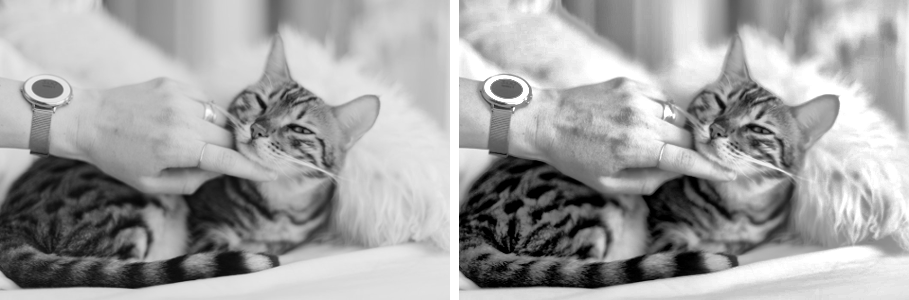
\includegraphics[width=0.95\textwidth]{img/cat.png}
  \caption{Left: input image. Right: sharpened image.}
\end{figure}

The cat's fur on the left-hand side, the person's hand and the cushion on the right-hand side appear to be more detailed.
We observe that the already sharp part of the image on the cat's head stays nice.
We obtained this filter by defining \(f(\Lapl) = -3\Lapl\) in the output image \(z = (I - f(\Lapl))y\).

This corresponds to the adaptive sharpening operator defined in \cite{siam_slides_2016} as \((I + \beta \Lapl)\) with \(\beta > 0\).
This approach remains a simple application of a scalar and doesn't require any eigenvalue computation.
A more complete approach is called multiscale decomposition \cite{talebi_nonlocal_2014} and consists of applying a polynomial function to the Laplacian \(\Lapl\).
We apply different coefficients to different eigenvalues of \(\Lapl\) because each eigenpair captures different features of the image.


\subsection{Approximate matrix computation}
As a reminder, we used GMRES to solve the linear systems with RAS preconditioning and using GMRES on the subdomains.
We sample 1\% of the pixels of an image with \(4 \cdot 10^5\) pixels using spatially uniform sampling.
The performances of the inverse subspace iteration for 50 and 500 eigenvalues:

\begin{figure}[H]
 \centering
 \begin{tikzpicture}
 \begin{groupplot}[
  group style={
   group size=2 by 1,
   xlabels at=edge bottom,
   ylabels at=edge left,
   horizontal sep=1.5cm,
   },
  height=6cm,
  width=0.5\textwidth,
  xlabel=Number of processors,
  xtick={2, 4, 8, 16, 32, 64, 128},
  xmode=log,
  ymode=log,
  log ticks with fixed point,
  ylabel=Runtime (seconds)
  ]
  \nextgroupplot[title={50 eigenvalues.}]
   \addplot[color=blue, mark=x] coordinates {
    (2, 772.1529408)
    (4, 381.4875584)
    (8, 196.6197338)
    (16, 104.6891928)
    (32, 59.8903464)
    (64, 35.9956886)
    (96, 29.214667)
    (128, 25.4793632)
    (160, 24.0418716)
    (192, 23.1824056)
   };

  \nextgroupplot[title={500 eigenvalues.}]
   \addplot[color=blue, mark=x] coordinates {
    (2, 7149.885403)
    (4, 5149.912356)
    (8, 4373.481026)
    (16, 3903.60577)
    (32, 3803.859549)
    (64, 3712.591258)
    (96, 3824.621957)
    (128, 3939.533307)
    (160, 3986.572888)
    (192, 4383.063958)
   };
 \end{groupplot}
\end{tikzpicture}

 \caption{Runtime of the inverse subspace iteration part of the algorithm (log scale).}
 \label{fig:inv_it_runtime}
\end{figure}

When increasing a low number of processors, we see an improvement of the performances in both cases of figure \ref{fig:inv_it_runtime}.
But the runtime stagnates slowly for 50 eigenvalues and quickly for 500 eigenvalues.
We even observe a raise of the runtime for 500 eigenvalues.
The algorithm reaches its parallelisation limit and the communication overhead takes over.
For 500 eigenvalues, the runtime for 2 processors is over 7000 seconds, and the fastest runtime is reached for 64 processors and is of 3700 seconds.

We know that the inverse iteration part of the algorithm is not scaling correctly compared to the other parts.
For any amount of computed eigenvalues, when we increase the number of processes, the proportion of time spent computing the eigenvalues increases.
For 500 eigenvalues and 128 processors, we spend more than 99\% of the time computing the eigenvalues.
This confirms that the algorithm does not quite scale yet.

We look at the internal steps of the inverse power method to see where lies the problem.
The algorithm consists of iteratively solving \(m\) linear systems, orthonormalising the vectors and computing the residual norm.
Here is the proportion of each step of the inverse subspace interation for the computation of 50 and 500 eigenvalues:

\begin{figure}[H]
 \centering
 \begin{tikzpicture}
 \begin{groupplot}[
  group style={
   group size=2 by 1,
   xlabels at=edge bottom,
   ylabels at=edge left,
   },
  ybar stacked,
  ymin=0,
  ymax=100,
  height=7cm,
  width=0.5\textwidth,
  xlabel=Number of processors,
  ylabel={Percentage (\%)},
  symbolic x coords={2, 4, 8, 16, 32, 64, 96, 128, 160, 192},
  legend style={
   at={(0, -0.25)},
   anchor=north}
  ]
  \nextgroupplot[title={50 eigenvalues.}]
  \addplot[ybar, fill=blue] plot coordinates {
   (2, 8.14)
   (4, 6.16)
   (8, 5.98)
   (16, 9.09)
   (32, 13.50)
   (64, 18.56)
   (96, 22.42)
   (128, 25.35)
   (160, 27.53)
   (192, 29.06)};
  \addplot[ybar, fill=red] plot coordinates {
   (2, 0.46)
   (4, 0.96)
   (8, 2.01)
   (16, 3.90)
   (32, 7.31)
   (64, 13.29)
   (96, 17.61)
   (128, 20.94)
   (160, 23.90)
   (192, 26.27)};
  \addplot[ybar, fill=yellow] plot coordinates {
   (2, 85.67)
   (4, 86.96)
   (8, 86.16)
   (16, 81.40)
   (32, 73.91)
   (64, 63.23)
   (96, 55.21)
   (128, 49.07)
   (160, 43.95)
   (192, 40.00)};
  \addplot[ybar, fill=green] plot coordinates {
   (2, 5.74)
   (4, 5.92)
   (8, 5.84)
   (16, 5.61)
   (32, 5.28)
   (64, 4.91)
   (96, 4.76)
   (128, 4.64)
   (160, 4.62)
   (192, 4.68)};

  \nextgroupplot[title={500 eigenvalues.}]
  \addplot[ybar, fill=blue] plot coordinates {
   (2, 23.76)
   (4, 15.29)
   (8, 11.43)
   (16, 12.30)
   (32, 11.68)
   (64, 9.84)
   (96, 9.47)
   (128, 9.75)
   (160, 9.57)
   (192, 9.39)};
  \addplot[ybar, fill=red] plot coordinates {
   (2, 46.02)
   (4, 63.07)
   (8, 75.14)
   (16, 79.65)
   (32, 83.37)
   (64, 86.81)
   (96, 87.72)
   (128, 87.77)
   (160, 88.07)
   (192, 88.50)};
  \addplot[ybar, fill=yellow] plot coordinates {
   (2, 28.78)
   (4, 20.15)
   (8, 11.97)
   (16, 6.60)
   (32, 3.49)
   (64, 1.84)
   (96, 1.29)
   (128, 0.98)
   (160, 0.80)
   (192, 0.64)};
  \addplot[ybar, fill=green] plot coordinates {
   (2, 1.44)
   (4, 1.48)
   (8, 1.46)
   (16, 1.46)
   (32, 1.46)
   (64, 1.51)
   (96, 1.53)
   (128, 1.50)
   (160, 1.56)
   (192, 1.47)};
  \legend{
   Solving the system of linear equations,
   Gram-Schmidt orthogonalisation,
   Residual norm computation,
   Rest overhead}
 \end{groupplot}
\end{tikzpicture}

 \caption{Proportion of each step in the inverse subspace iteration.}
 \label{fig:inv_it_proportion}
\end{figure}

We observe from figure \ref{fig:inv_it_proportion} that the Gram-Schmidt orthogonalisation is the limiting factor and is the most time-consuming step of the inverse iteration as the number of processors grows.
It is a well-known problem that the simple Gram-Schmidt process is actually difficult to parallelise efficiently.
Small optimisations for a parallel Gram-Schmidt orthogonalisation exist \cite{katagiri_parallel_gram_schmidt_2003} but they do not properly solve the problem.
This issue will be difficult to overcome completely.


\subsection{Skipping some orthogonalisations}
Fundamentally, the orthogonalisation is used to stabilise the algorithm.
To accelerate our algorithm further, we try to orthogonalise the vectors \(X_k\) every other iteration instead of every iteration.
We present below the resulting performances:

\begin{figure}[H]
  \centering
  \begin{tikzpicture}
 \begin{groupplot}[
  group style={
   group size=2 by 1,
   xlabels at=edge bottom,
   ylabels at=edge left,
   horizontal sep=1.5cm,
   },
  height=6cm,
  width=0.5\textwidth,
  xlabel=Number of processors,
  xtick={2, 4, 8, 16, 32, 64, 128},
  xmode=log,
  ymode=log,
  log ticks with fixed point,
  ylabel=Runtime (seconds)
  ]
  \nextgroupplot[title={50 eigenvalues.}]
   \addplot[color=blue, mark=x] coordinates {
    (2, 819.1718588)
    (4, 404.5779052)
    (8, 207.887785)
    (16, 109.2656354)
    (32, 61.5224218)
    (64, 35.5858806)
    (96, 28.0760846)
    (128, 24.3417164)
    (160, 22.365463)
    (192, 21.1874868)
   };

  \nextgroupplot[title={500 eigenvalues.}]
   \addplot[color=blue, mark=x] coordinates {
    (2, 5613.950337)
    (4, 3614.57139)
    (8, 2804.417351)
    (16, 2346.925115)
    (32, 2223.999989)
    (64, 2104.544023)
    (96, 2148.624336)
    (128, 2264.674778)
    (160, 2226.515463)
    (192, 2494.121987)
   };
 \end{groupplot}
\end{tikzpicture}

  \caption{Runtime of the inverse subspace iteration with skipping the Gram-Schmidt procedure every other iteration (log scale).}
\end{figure}

The performances for 50 eigenvalues are similar to the case when we are not skipping the Gram-Schmidt orthogonalisation every other iteration.
We saw that only a small proportion of time is spent doing the orthogonalisation in this case, so the impact is not significant.

However, for computing 500 eigenvalues, the runtime with skipping the orthogonalisation every other iteration is much lower.
Most time is spent doing the Gram-Schmidt process, so the execution is considerably sped up.
For 2 processors, the runtime is around 5600 seconds and the fastest runtime is 2100 seconds for 64 processors.
Even if the algorithm requires a few more outer iterations to converge, we nearly observe a factor 2 speed up with respect to the algorithm without skipping the Gram-Schmidt procedure.
The communication overhead of the method remains a problem when the number of processors is large.

When skipping the Gram-Schmidt more often than every other iteration, we might see further improvements.
Below the runtime for 2 and 64 processors of the inverse subspace algorithm depending on the frequency of orthogonalisation:

\begin{figure}[H]
  \centering
  \begin{tikzpicture}
 \begin{groupplot}[
  group style={
   group size=2 by 1,
   xlabels at=edge bottom,
   ylabels at=edge left,
   horizontal sep=2.2cm,
   },
  height=6cm,
  width=0.5\textwidth,
  xlabel={Orthogonalisation every \(x\) iterations},
  xtick={1, 2, 3, 4, 5},
  %xmode=log,
  %ymode=log,
  %log ticks with fixed point,
  ylabel=Runtime (seconds),
  legend style={
   at={(1, -0.3)},
   anchor=north
  },
  ]
  \nextgroupplot[title={2 processors, 500 eigenvalues.}]
   \addplot[color=blue, mark=x] coordinates {
    (1, 7149.885403)
    (2, 5613.950337)
    (3, 0)
    (4, 0)
    (5, 0)
   };
   \addlegendentry{Runtime}
   \addplot[color=black, domain=1:5, dashed] expression {
    7149.885403/x};
   \addlegendentry{Linear speedup}

  \nextgroupplot[title={64 processors, 500 eigenvalues.}]
   \addplot[color=blue, mark=x] coordinates {
    (1, 3712.591258)
    (2, 2104.544023)
    (3, 0)
    (4, 0)
    (5, 0)
   };
   \addplot[color=black, domain=1:5, dashed] expression {
    3712.591258/x};
 \end{groupplot}
\end{tikzpicture}


  \caption{Runtime of the inverse subspace iteration depending on the amount of Gram-Schmidt procedures.}
\end{figure}

For 2 processors, we see that the speedup stagnates quickly when skipping the Gram-Schmidt orthogonalisation more and more often.
Indeed, the orthogonalisation represents a decent proportion of the execution time for 2 processors whereas it represents over 85\% for 64 processors.
Therefore we observe a speedup of the inverse subspace iteration that is nearly linear for 64 processors.
The number of outer iterations between not skipping the Gram-Schmidt algorithm and applying it every 5 iterations only varies from 38 to 40 which explains the resulting runtime.


\section{Conclusion}

\subsection{Discussions}
\paragraph{Linear solvers \& domain decomposition methods on dense matrices}
The presented experiments show that the resolution of linear systems scales with respect to the number of processors.
Domain decomposition methods improve the performances of solving dense systems of linear equations, even without overlap, in the context of image processing.
Indeed, these methods are naturally parallel and precondition the matrix appropriately.
This becomes clear when observing the performances improvement on large matrices.

\ifthesis
 In the case of a small input image, a direct solver shows the best results for computing the inverses for preconditioning.
 On larger inputs, these are not available but using iterative Krylov type methods on the subdomains also exposes a considerable improvement compared to the case without preconditioner.
\fi

\paragraph{Gram-Schmidt process}
The orthogonalisation process is difficult to parallelise efficiently.
\ifthesis
 Skipping the Gram-Schmidt procedure every other iteration, to stabilise the algorithm less often, gave an improvement, but we cannot totally avoid the cost of it when increasing the number of processors.
 Skipping the Gram-Schmidt procedure more often tends to improve the runtime when a large amount of processors is involved.
\else
 Skipping the Gram-Schmidt procedure tends to improve the runtime when a large amount of processors is involved.
\fi
However, the stability of the algorithm diminishes when omitting numerous orthogonalisations.
This scalability problem is well-known and one of the biggest limitations for scaling diverse algorithms to a large number of processors.

The Gram-Schmidt procedure orthogonalises a set of vectors by sequentially substracting from a vector the projections on the previously orthogonalised vectors.
The inner product of two vectors is computed frequently, because of the projection, and since each vector is shared over all processors, a lot of communication is involved in this operation.
Attempts for parallel implementation are numerous, like \cite{katagiri_parallel_gram_schmidt_2003}, but they either still have many communications or suggest a different memory distribution schema.


\subsection{Perspectives}
\paragraph{Image processing}
Numerous possibilities for improving the algorithm result from the applied simplifications.
An important matter would be to complete the final part of the algorithm computing the output image.
This requires to compute the inverse of the square root of the matrix.
\ifthesis
 This can be done either by calculating the entire eigendecomposition to get the inverse square root matrix.
 Another way to accomplish this, could be to consider Cauchy's integral formula such as:
 \[A^{-\frac{1}{2}} = \frac{1}{2\pi i} \oint_C z^{-\frac{1}{2}} (zI - A)^{-1} \mathrm{d}z.\]
 However, the time for this project was not sufficient to explore this possibility entirely.

 An easy improvement to make such an algorithm production ready, would be to consider color images.
 This can be done by decomposing the RGB image to a YCC image, with one grayscale and two chroma components.
 The algorithm is applied to all three components, and then they are converted back to RGB.
\fi

A way to improve the filtering is multiscale decomposition.
As explained in \cite{talebi_nonlocal_2014}, instead of applying a linear function to all eigenvalues such as \(f(W) = \phi f(\Pi) \phi^T\), we can actually use a polynomial function \(f\).
This is interesting because each eigenpair captures various features of the image and one can apply different coefficients on different aspects of the image.

For the state-of-the-art, the article \cite{talebi_fast_2016} proposes an enhancement of global filtering.
They argue that the eigendecomposition remains computationally too expensive and show results of an improvement.
The presented results and performances are astonishing; however, the method is hardly described and replicating it would be difficult.
This is understandable since this algorithm seems to be in the latest Pixel 2 smartphone by Google and they surely want to preserve their market advantage in the field of image processing.

\paragraph{}
An improvement of the algorithm of the present case, would be to formulate a method for extending the trailing eigenvectors of the sampled Laplacian \(\Lapl_A\) and not only the leading ones as the Nystr\"om extension supports.
This way, it would be possible to apply the spectral decomposition of the Laplacian, and thus apply a filter to the input image, avoiding the computation of the inverse square root of the matrix.

\ifthesis
 \paragraph{Linear solver}
 A way to highly parallelise the matrix computations could be using graphical processing units (GPUs).
 Especially the matrix-matrix and matrix-vector products could be nicely improved with GPUs.
 However, solving systems of linear equations is a task that GPUs are not designed for.

 \paragraph{}
 It also would be interesting to explore more the impact of the number of sampled pixels, which corresponds to the input matrix of the linear system.
 The articles \cite{fowlkes_spectral_2004} and \cite{glide_2014} started a study on the size of the samples, but only for small images.
 This work could be extended.
\fi

To conclude, various possibilities remain to be exploited by future work.


\printbibliography

\end{document}
